\chapter{ETL and Unified Database}
\minitoc
\clearpage

\section{Introduction}
This chapter presents Sprint 3, focused on building the ETL foundation and the unified operational database. The goal was to bring data from different systems into one clean, consistent, and monitorable flow before using it in business modules.

\section{Sprint Backlog}
The sprint backlog for Sprint 3 was formalized as user stories focused on ETL and unified database delivery:

\begin{center}
\renewcommand{\arraystretch}{1.2}
\begin{tabular}{|l|>{\raggedright\arraybackslash}p{9.0cm}|l|}
\hline
\textbf{ID} & \textbf{User Story} & \textbf{Priority} \\
\hline
US1 & As a system administrator, I want to connect to BioTime and EasyProject data sources so that ETL can extract operational data. & High \\
\hline
US2 & As a data engineer, I want to build entity-based extraction pipelines (departments, employees, attendance, projects, members) to structure ingestion. & High \\
\hline
US3 & As a data engineer, I want to apply transformation and normalization rules so that unified data remains clean and consistent. & High \\
\hline
US4 & As a system, I want to load transformed records into the PostgreSQL target schema while preserving referential integrity. & High \\
\hline
US5 & As an administrator, I want to monitor ETL execution status and errors in real time so that failures can be detected early. & Medium \\
\hline
\end{tabular}
\end{center}

\section{Sprint Design}
Sprint design followed an ETL-first approach. We apply integrity and control rules before application services consume the data.

\subsection{Refinement of data rules and ETL mappings}
At this stage, we refined the mapping rules between BioTime and EasyProject so the data could be loaded in a clean and consistent way. We aligned identifiers, normalized data types, and handled common conflicts between the two sources. We also paid special attention to duplicates, attendance consistency, and the loading order between related entities.
\section{Conception}

\subsection{ETL Pipeline Architecture}
The ETL process uses a modular and scalable architecture. This design improves maintainability, traceability, and consistency in the unified database.

\subsubsection*{1. Data Sources}
Data is extracted from two main external systems:
\begin{itemize}[noitemsep]
    \item \textbf{BioTime}: attendance and employee activity data.
    \item \textbf{EasyProject}: project and member-related data.
\end{itemize}
The extraction layer uses \textbf{SQLAlchemy (Async ORM)} for efficient asynchronous communication with source databases.

\subsubsection*{2. Modular Pipeline Design}
To keep responsibilities clear and reusable, the ETL process is split into independent pipelines. Each pipeline handles one entity:
\begin{itemize}[noitemsep]
    \item Departments pipeline
    \item Employees pipeline
    \item Attendance pipeline
    \item Projects pipeline
    \item Members pipeline
    \item Attendance events pipeline
    \item Employee attendance events pipeline
\end{itemize}
Each pipeline handles extraction, transformation (cleaning, mapping, normalization), and loading into the unified target database.

Figure~\ref{fig:modular-etl-architecture} shows how independent pipeline modules separate extraction, transformation, and loading responsibilities.

\begin{figure}[H]
\caption{Modular ETL architecture built around entity-based pipelines}
\label{fig:modular-etl-architecture}
\centering
\IfFileExists{diagrams/ch3-modular-etl-architecture.png}{%
    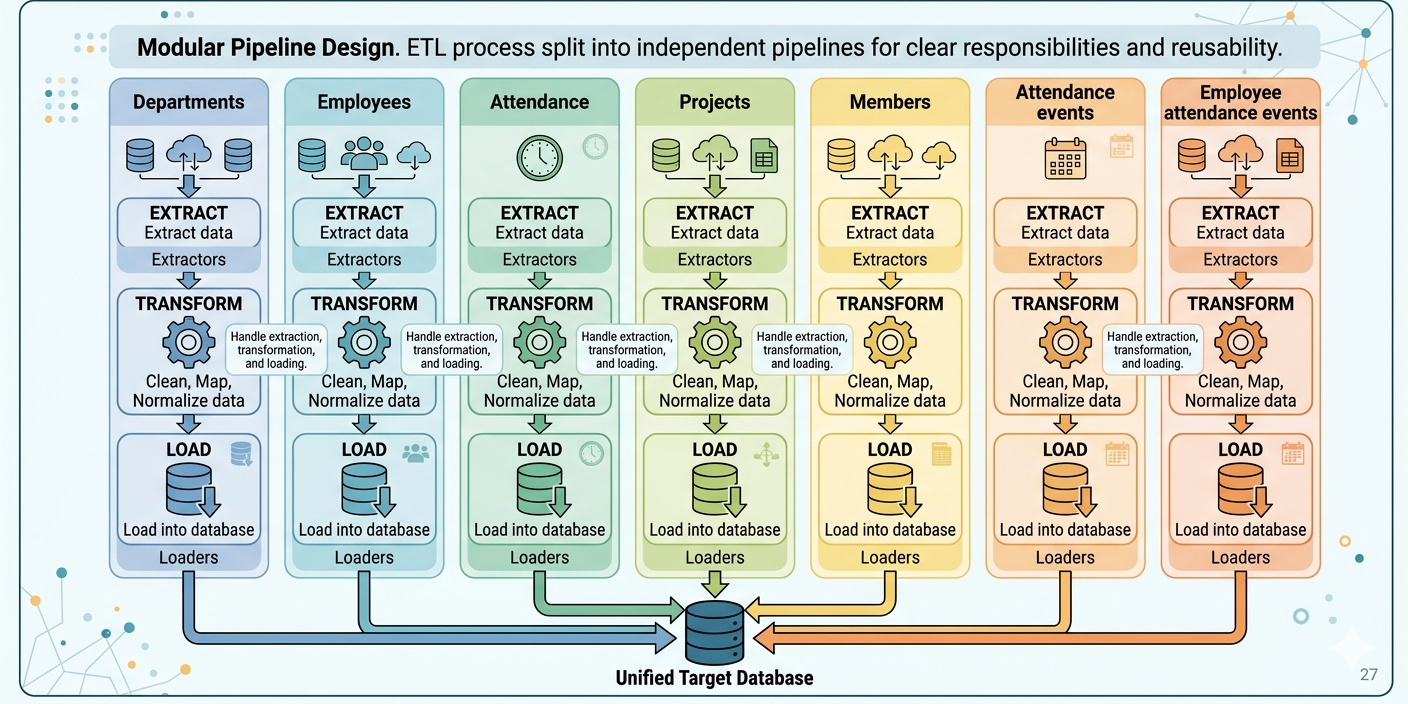
\includegraphics[width=0.92\textwidth,height=0.52\textheight,keepaspectratio]{diagrams/ch3-modular-etl-architecture.png}
}{%
    \fbox{\parbox{0.9\textwidth}{
    \centering
    \vspace{1.6cm}
    \textit{Missing file: diagrams/ch3-modular-etl-architecture.png}\\
    \textit{Insert modular ETL architecture diagram (extractors/loaders/pipelines).}
    \vspace{1.6cm}
    }}
}
\end{figure}


\subsubsection*{3. Orchestration via Main Pipeline}
The Main Pipeline orchestrates all ETL pipelines in a strict predefined order. This order must stay unchanged to preserve referential integrity and avoid loading conflicts.

\textbf{Execution flow:}
\begin{enumerate}[noitemsep]
    \item Truncate target tables using \texttt{TRUNCATE ... CASCADE} to start from a clean load state.
    \item Run pipelines in sequence: Departments $\to$ Employees $\to$ Attendance $\to$ Projects $\to$ Members $\to$ Attendance Events $\to$ Employee Attendance Events.
    \item Return final execution status and total processing time.
\end{enumerate}

Figure~\ref{fig:main-pipeline-sequence} details truncation, ordered pipeline execution, and final completion reporting.

\begin{figure}[H]
\caption{Sequence of the main pipeline orchestration}
\label{fig:main-pipeline-sequence}
\centering
\IfFileExists{diagrams/ch3-main-pipeline-sequence.png}{%
    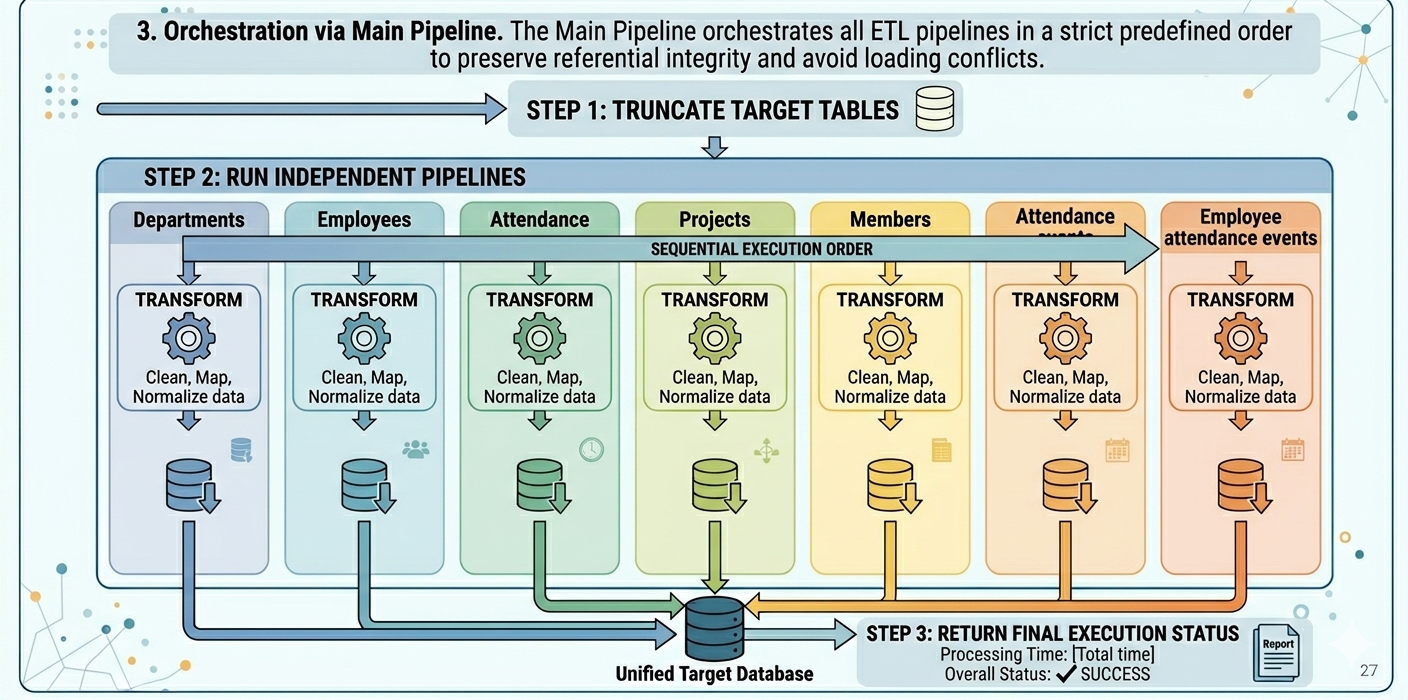
\includegraphics[width=0.92\textwidth,height=0.50\textheight,keepaspectratio]{diagrams/ch3-main-pipeline-sequence.png}
}{%
    \fbox{\parbox{0.9\textwidth}{
    \centering
    \vspace{1.6cm}
    \textit{Missing file: diagrams/ch3-main-pipeline-sequence.png}\\
    \textit{Insert main pipeline orchestration sequence diagram.}
    \vspace{1.6cm}
    }}
}
\end{figure}


\subsubsection*{4. Asynchronous Streaming with FastAPI}
The Main Pipeline is implemented with an asynchronous generator in FastAPI to stream progress in real time.

\textbf{Key features:}
\begin{itemize}[noitemsep]
    \item A status update is emitted for each ETL step.
    \item Execution time is measured per step.
    \item Errors are captured and returned immediately.
\end{itemize}

Example streamed payload:
\begin{verbatim}
{
  "step": "employees",
  "status": "finished",
  "time": 1.23
}
\end{verbatim}

\subsubsection*{5. Real-Time Monitoring Interface}
The ETL workflow is integrated through the FastAPI backend and exposed in the Admin settings page on the frontend. This lets administrators monitor execution in real time, detect slow or failing steps, and keep full visibility over the integration process.

\subsection{Data Validation and Control Flow}
To guarantee data quality and consistency, we implemented several validation and control mechanisms:

\subsubsection*{1. Data Validation}
\begin{itemize}[noitemsep]
    \item Verify required fields before insertion.
    \item Normalize data types.
    \item Handle missing or inconsistent values.
\end{itemize}

\subsubsection*{2. Referential Integrity}
Dependencies are preserved through strict pipeline order (for example, employee records depend on department records).

\subsubsection*{3. Error Handling}
A protected try/catch orchestration flow captures failures, streams error details to the client, and raises HTTP exceptions when needed.

\subsubsection*{4. Performance Monitoring}
Execution time is measured with \texttt{time.perf\_counter()} for each step to identify bottlenecks and support optimization.

Figure~\ref{fig:validation-control-flow} summarizes validation checkpoints, dependency enforcement, error propagation, and performance tracking.

\begin{figure}[H]
\caption{Data validation and control-flow mechanisms used in the ETL process}
\label{fig:validation-control-flow}
\centering
\IfFileExists{diagrams/ch3-validation-control-flow.png}{%
    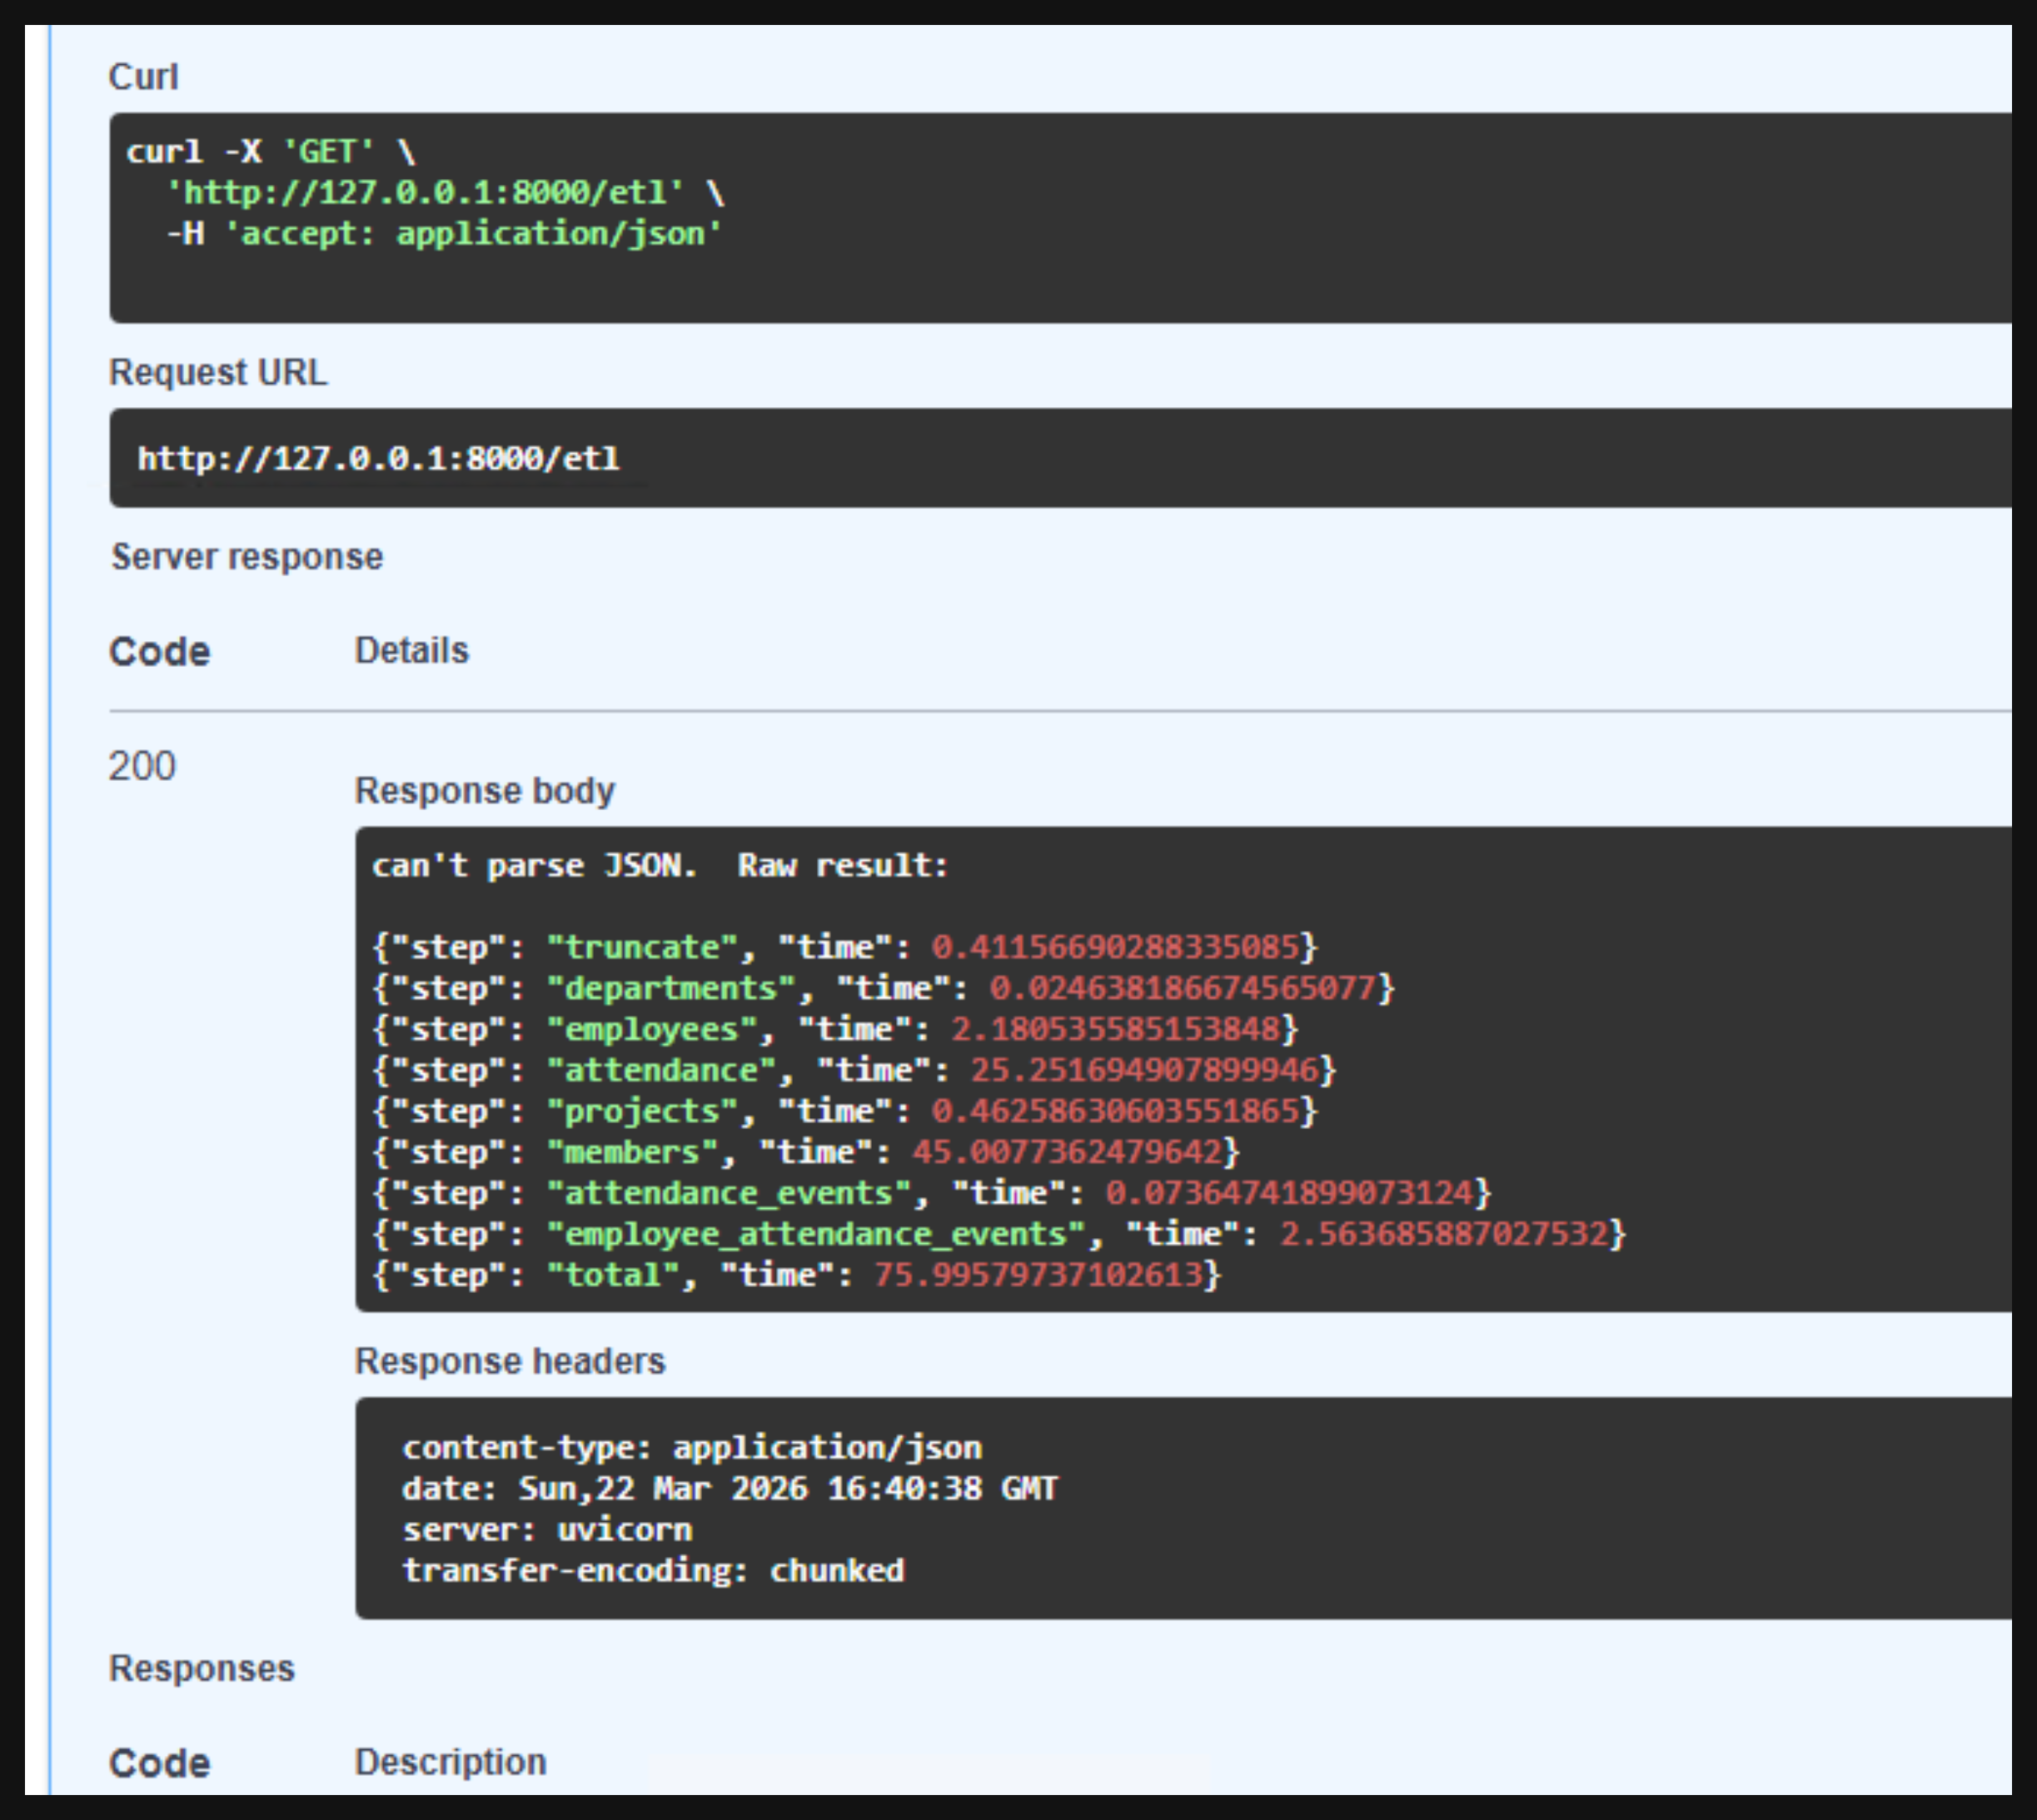
\includegraphics[width=0.92\textwidth,height=0.48\textheight,keepaspectratio]{diagrams/ch3-validation-control-flow.png}
}{%
    \fbox{\parbox{0.9\textwidth}{
    \centering
    \vspace{1.6cm}
    \textit{Missing file: diagrams/ch3-validation-control-flow.png}\\
    \textit{Insert validation and control-flow diagram.}
    \vspace{1.6cm}
    }}
}
\end{figure}


\subsection{Key Design Advantages}
\begin{itemize}[noitemsep]
    \item \textbf{Modularity}: easier maintenance and extension.
    \item \textbf{Scalability}: new pipelines can be added with low coupling.
    \item \textbf{Observability}: ETL progress is streamed in real time.
    \item \textbf{Data Integrity}: controlled execution order prevents conflicts.
    \item \textbf{Performance Awareness}: per-step timing supports optimization.
\end{itemize}

\section{Sprint Realization}
\subsection{Implementation outcomes}
\begin{itemize}[noitemsep]
    \item Implemented source extractors and entity-based ETL pipelines.
    \item Implemented a main orchestrator with ordered execution and full-table refresh strategy.
    \item Integrated asynchronous streaming logs into backend endpoints and the admin monitoring UI.
    \item Applied validation, error handling, and execution-time tracking across ETL steps.
\end{itemize}

\section{Conclusion}
Sprint 3 delivered a robust and observable ETL foundation and produced the unified PostgreSQL database used by later modules. The resulting data layer ensures consistency, traceability, and operational readiness for authentication, HR, and project-management features.
